\documentclass[12pt]{article}
%%---------------------------------------------------------------------
% packages
% geometry
\usepackage{geometry}
% font
\usepackage{fontspec}
\defaultfontfeatures{Mapping=tex-text}  %%如果没有它,会有一些 tex 特殊字符无法正常使用,比如连字符。
\usepackage{xunicode,xltxtra}
\usepackage[BoldFont,SlantFont,CJKnumber,CJKchecksingle]{xeCJK}  % \CJKnumber{12345}: 一万二千三百四十五
\usepackage{CJKfntef}  %%实现对汉字加点、下划线等。
\usepackage{pifont}  % \ding{}
% math
\usepackage{amsmath,amsfonts,amssymb}
% color
\usepackage{color}
\usepackage{xcolor}
\definecolor{EYE}{RGB}{199,237,204}
\definecolor{FLY}{RGB}{128,0,128}
\definecolor{ZHY}{RGB}{139,0,255}
% graphics
\usepackage[americaninductors,europeanresistors]{circuitikz}
\usepackage{tikz}
\usetikzlibrary{positioning,arrows,shadows,shapes,calc,mindmap,trees,backgrounds}  % placements=positioning
\usepackage{graphicx}  % \includegraphics[]{}
\usepackage{subfigure}  %%图形或表格并排排列
% table
\usepackage{colortbl,dcolumn}  %% 彩色表格
\usepackage{multirow}
\usepackage{multicol}
\usepackage{booktabs}
% code
\usepackage{fancyvrb}
\usepackage{listings}
% title
\usepackage{titlesec}
% head/foot
\usepackage{fancyhdr}
% ref
\usepackage{hyperref}
% pagecolor
\usepackage[pagecolor={EYE}]{pagecolor}
% tightly-packed lists
\usepackage{mdwlist}

\usepackage{styles/iplouccfg}
\usepackage{styles/zhfontcfg}
\usepackage{styles/iplouclistings}

%%---------------------------------------------------------------------
% settings
% geometry
\geometry{left=2cm,right=1cm,top=2cm,bottom=2cm}  %设置 上、左、下、右 页边距
\linespread{1.5} %行间距
% font
\setCJKmainfont{Adobe Kaiti Std}
%\setmainfont[BoldFont=Adobe Garamond Pro Bold]{Apple Garamond}  % 英文字体
%\setmainfont[BoldFont=Adobe Garamond Pro Bold,SmallCapsFont=Apple Garamond,SmallCapsFeatures={Scale=0.7}]{Apple Garamond}  %%苹果字体没有SmallCaps
\setCJKmonofont{Adobe Fangsong Std}
% graphics
\graphicspath{{figures/}}
\tikzset{
    % Define standard arrow tip
    >=stealth',
    % Define style for boxes
    punkt/.style={
           rectangle,
           rounded corners,
           draw=black, very thick,
           text width=6.5em,
           minimum height=2em,
           text centered},
    % Define arrow style
    pil/.style={
           ->,
           thick,
           shorten <=2pt,
           shorten >=2pt,},
    % Define style for FlyZhyBall
    FlyZhyBall/.style={
      circle,
      minimum size=6mm,
      inner sep=0.5pt,
      ball color=red!50!blue,
      text=white,},
    % Define style for FlyZhyRectangle
    FlyZhyRectangle/.style={
      rectangle,
      rounded corners,
      minimum size=6mm,
      ball color=red!50!blue,
      text=white,},
    % Define style for zhyfly
    zhyfly/.style={
      rectangle,
      rounded corners,
      minimum size=6mm,
      ball color=red!25!blue,
      text=white,},
    % Define style for new rectangle
    nrectangle/.style={
      rectangle,
      draw=#1!50,
      fill=#1!20,
      minimum size=5mm,
      inner sep=0.1pt,}
}
\ctikzset{
  bipoles/length=.8cm
}
% code
\lstnewenvironment{VHDLcode}[1][]{%
  \lstset{
    basicstyle=\footnotesize\ttfamily\color{black},%
    columns=flexible,%
    framexleftmargin=.7mm,frame=shadowbox,%
    rulesepcolor=\color{blue},%
%    frame=single,%
    backgroundcolor=\color{yellow!20},%
    xleftmargin=1.2\fboxsep,%
    xrightmargin=.7\fboxsep,%
    numbers=left,numberstyle=\tiny\color{blue},%
    numberblanklines=false,numbersep=7pt,%
    language=VHDL%
    }\lstset{#1}}{}
\lstnewenvironment{VHDLmiddle}[1][]{%
  \lstset{
    basicstyle=\scriptsize\ttfamily\color{black},%
    columns=flexible,%
    framexleftmargin=.7mm,frame=shadowbox,%
    rulesepcolor=\color{blue},%
%    frame=single,%
    backgroundcolor=\color{yellow!20},%
    xleftmargin=1.2\fboxsep,%
    xrightmargin=.7\fboxsep,%
    numbers=left,numberstyle=\tiny\color{blue},%
    numberblanklines=false,numbersep=7pt,%
    language=VHDL%
    }\lstset{#1}}{}
\lstnewenvironment{VHDLsmall}[1][]{%
  \lstset{
    basicstyle=\tiny\ttfamily\color{black},%
    columns=flexible,%
    framexleftmargin=.7mm,frame=shadowbox,%
    rulesepcolor=\color{blue},%
%    frame=single,%
    backgroundcolor=\color{yellow!20},%
    xleftmargin=1.2\fboxsep,%
    xrightmargin=.7\fboxsep,%
    numbers=left,numberstyle=\tiny\color{blue},%
    numberblanklines=false,numbersep=7pt,%
    language=VHDL%
    }\lstset{#1}}{}
% pdf
\hypersetup{pdfpagemode=FullScreen,%
            pdfauthor={Haiyong Zheng},%
            pdftitle={Title},%
            CJKbookmarks=true,%
            bookmarksnumbered=true,%
            bookmarksopen=false,%
            plainpages=false,%
            colorlinks=true,%
            citecolor=green,%
            filecolor=magenta,%
            linkcolor=cyan,%red(default)
            urlcolor=cyan}
% section
%http://tex.stackexchange.com/questions/34288/how-to-place-a-shaded-box-around-a-section-label-and-name
\newcommand\titlebar{%
\tikz[baseline,trim left=3.1cm,trim right=3cm] {
    \fill [cyan!25] (2.5cm,-1ex) rectangle (\textwidth+3.1cm,2.5ex);
    \node [
        fill=cyan!60!white,
        anchor= base east,
        rounded rectangle,
        minimum height=3.5ex] at (3cm,0) {
        \textbf{\thesection.}
    };
}%
}
\titleformat{\section}{\Large\bf\color{blue}}{\titlebar}{0.1cm}{}
% head/foot
\setlength{\headheight}{15pt}
\pagestyle{fancy}
\fancyhf{}
%\lhead{\color{black!50!green}2014年秋季学期}
\chead{\color{black!50!green}显著性检测}
%\rhead{\color{black!50!green}通信电子电路}
\lfoot{\color{blue!50!green}朱亚菲}
\cfoot{\color{blue!50!green}\href{http://vision.ouc.edu.cn/~zhenghaiyong}{CVBIOUC}}
\rfoot{\color{blue!50!green}$\cdot$\ \thepage\ $\cdot$}
\renewcommand{\headrulewidth}{0.4pt}
\renewcommand{\footrulewidth}{0.4pt}


%%---------------------------------------------------------------------
\begin{document}
%%---------------------------------------------------------------------
%%---------------------------------------------------------------------
% \titlepage
\title{\vspace{-2em}显著性检测\vspace{-0.7em}}
\author{朱亚菲}
\date{\vspace{-0.7em}2015年2月\vspace{-0.7em}}
%%---------------------------------------------------------------------
\maketitle\thispagestyle{fancy}
%%---------------------------------------------------------------------
\maketitle
\tableofcontents 

\section{引言}

由论文“A closer look at context: from coxes to the contextual emergence of object saliency”知道


\section{多尺度的概念}

多尺度

\section{Hierarchical Saliency Detection}

这篇论文主要解决的是当图像中显著前景或背景中存在小尺度大对比度patterns,而在生成的显著图中并不突出这些patterns的情况。论文框架如图~\ref{fig: hsaliency1}。主要步骤是三步:首先从原图像中提取layers,然后从每个layer中计算saliency cues,最后把它们融入一个分层模型以得到最终的结果。

\begin{figure}[!ht]
\centering
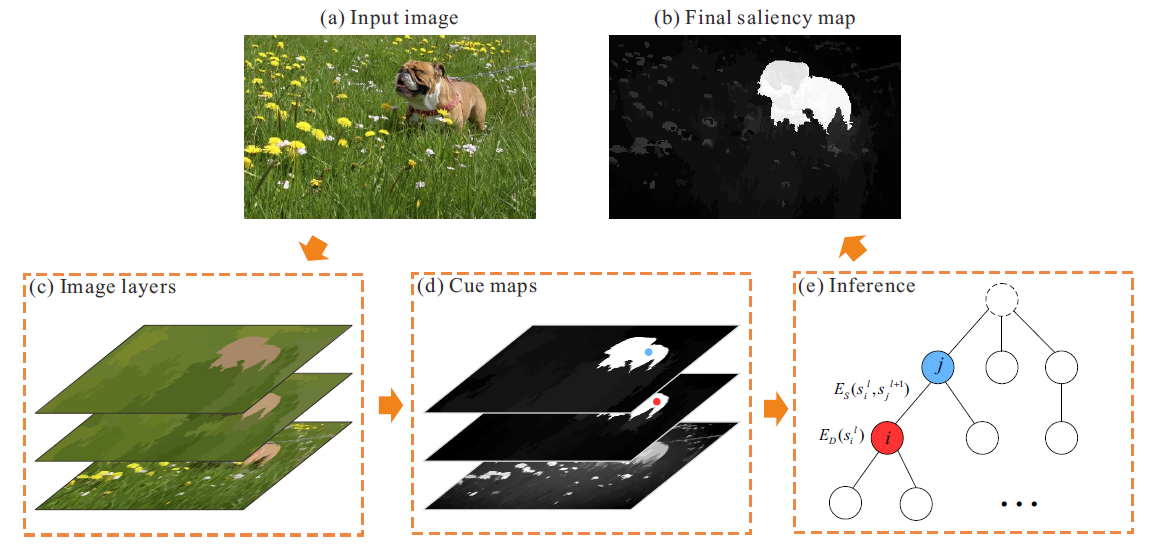
\includegraphics[width=0.8\textwidth]{hsaliency1.png}
\caption{框架}
\label{fig: hsaliency1}
\end{figure} 

分层与多尺度、多分辨率的区别?

1. 如何提取这三个layers?如图~\ref{fig: hsaliency2}

\begin{figure}[!ht]
\centering
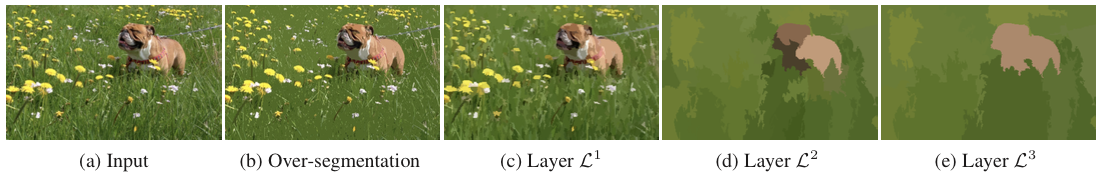
\includegraphics[width=0.85\textwidth]{hsaliency2.png}
\caption{不同尺度下的区域合并结果}
\label{fig: hsaliency2}
\end{figure}

先对原图像($400 \times 300$)用watershed-like方法~\cite{gonzalez2009digital}进行初始的过分割,对每个分割区域计算一个scale值,然后对所有区域的scale值按从小到大排序,如果一个区域的scale值小于3,就将它和最近的区域合并(通过判断两个区域内CIELUV颜色均值的距离),然后更新它的scale,并更新合并区域的颜色均值,等对所有区域都处理后,得到的结果就是$L^1$层。$L^2$层是通过对$L^1$层采取同样的步骤,只不过用一个更大的阈值17。$L^3$层也是如此,阈值取33。

2. 如何求每个区域的scale?

通常在Mean shift、graph-based segmentation等超像素分割方法中,区域的size是指该区域内所有像素的个数。本论文指出了这样的不合理性,就人类视觉感知而言,较多的像素个数和大尺度的区域并不完全符合。如图~\ref{fig: hsaliency3},尽管弯曲的区域a包含了很多像素,但对于我们的视觉感受却并不觉得它很大,而b看着会更大一些,尽管它的像素个数并不是很多。根据这样的现象,作者基于shape uniformities定义了一个新的encompassment scale measure,以用来在合并阶段获取区域的size。

\begin{figure}[!ht]
\centering
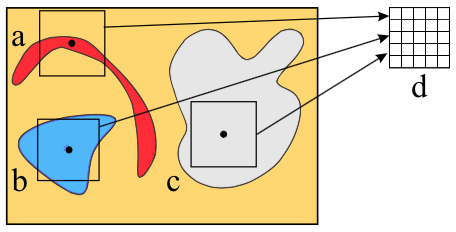
\includegraphics[width=0.4\textwidth]{hsaliency3.png}
\caption{scale}
\label{fig: hsaliency3}
\end{figure}

关于scale的定义如下:
\begin{align}
scale(R) == arg \max_i {R_{t \times t}|R_{t \times t} \subseteq R}
\end{align}

其中,$R_{t \times t}$是一个$t \times t$的正方形区域。也就是说,一个区域的scale是指该区域内所能包含的最大方形区域的边长。这里并不需要通过复杂的计算来算出每个区域的scale是多大,只要判断其相对于阈值是大还是小,这样就简化了,可以对每个区域用一个$t \times t$的模板进行滤波,如果滤完后该区域内所有像素值都被更新了,说明该区域的scale小于t,反之说明大于t,如图~\ref{fig: hsaliency4}所示。

\begin{figure}[!ht]
\centering
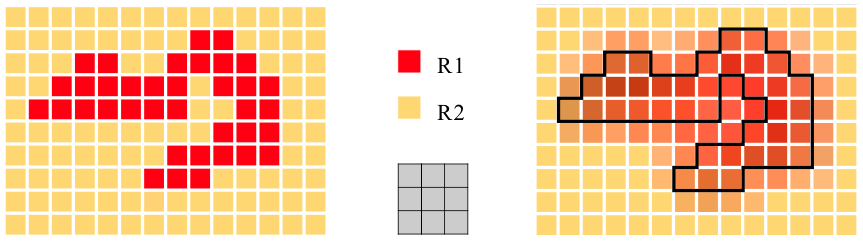
\includegraphics[width=0.6\textwidth]{hsaliency4.png}
\caption{scale}
\label{fig: hsaliency4}
\end{figure}

3. 如何计算每一层的saliency cues?

主要从颜色、位置、大小三个方面提取saliency cues,以找到该层比较重要的pixels,作者用了两种cues:

1)local contrast

\begin{align}
C_i = \sum_{j=1}^{n}w(R_i)\Phi(i, j)||c_i-c_j||_2
\end{align}


2)location heuristic

心理物理学方面的研究表示人类视觉注意偏好图像的中央区域,所以在通常情况下越靠近图像中央的像素越显著。
\begin{align}
H_i = \frac{1}{w(R_i)}\sum_{x_i \in R_i} exp\{-\lambda||x_i-x_c||^2\}
\end{align}

然后将$C_i$与$H_i$组合起来,得到
\begin{align}
\bar{s}_i = C_i \cdot H_i
\end{align}

由于local contrast和location cues都被归一化到$[0, 1)$,它们各自的重要性由$\lambda$来控制。当对三个layers均计算完$\bar{s}_i$后,就可以得到每一层的初始显著图,最后通过一种hierarchical inference procedure来对多尺度显著性检测结果进行融合。

4. 最后一步Hierarchical Inference是怎么进行的?

Cue maps显示了不同尺度下的显著性,效果很不一样。在底层,会产生很多小区域,而在高层会包含大尺度的结构。由于图像的多样性,单独的一层并不能保证效果是完美的,也很难判别哪一层是效果最好的。

由于背景或前景的复杂性,单纯通过求这三层产生的显著图的平均值来融合并不是一个好的选择。作者构造了一个基于树结构的图,见图~\ref{fig: hsaliency1}中的(e),其中的节点代表相应层中的区域。节点$j$在下一层中包含两个分割区域,因而有两个子节点。其中父节点代表整幅图像的最粗糙表示。

将图中对应于第$L_l$层中第$i$个区域的节点上的显著性定义为变量$s_i^l$,设$S$是包含图中所有节点的集合。最小化如下的能量方程:
\begin{align}
E(S) = \sum_l \sum_i E_D(s_i^l)+\sum_l \sum_{i, R_i^l \subseteq R_j ^{l+1}} E_S(s_i^l, s_j^{l+1})
\end{align}

%
% references
\bibliographystyle{plain}

\bibliography{saliency} %参考文献


\end{document}